\setcounter{section}{2}
\section{HÀM SỐ LƯỢNG GIÁC VÀ ĐỒ THỊ}
\subsection{KIẾN THỨC CẦN NHỚ}
\subsubsection{Hàm số chẵn, hàm số lẻ}
\indam{Định nghĩa:}
Cho hàm số $y=f(x)$ có tập xác định là $\mathscr{D}$.
\begin{itemize}
	\item Hàm số $f(x)$ được gọi là \textbf{hàm số chẵn} nếu $\forall x \in \mathscr{D}$ thì $-x \in \mathscr{D}$ và $f(-x)=f(x)$. Đồ thị của một hàm số chẵn nhận trục tung là trục đối xứng.
	\item Hàm số $f(x)$ được gọi là \textbf{hàm số lẻ} nếu $\forall x \in \mathscr{D}$ thì $-x \in \mathscr{D}$ và $f(-x)=-f(x)$. Đồ thị của một hàm số lẻ nhận gốc toạ độ là tâm đối xứng.
\end{itemize}
% \subsubsection{Hàm số tuần hoàn}
% \indamm{Định nghĩa}
% 	Hàm số $y=f(x)$ có tập xác định $\mathscr{D}$ được gọi là \textbf{hàm số tuần hoàn} nếu tồn tại số $T \neq 0$ sao cho với mọi $x \in \mathscr{D}$ ta có:
% 	\begin{enumerate}[i)]
% 		\item $x+T \in \mathscr{D}$ và $x-T \in \mathscr{D}$;
% 		\item $f(x+T)=f(x)$.
% 	\end{enumerate}
% 	Số $T$ dương nhỏ nhất thỏa mãn các điều kiện trên (nếu có) được gọi là \textbf{chu kì} của hàm số tuần hoàn đó.

% \begin{nx}
% 	 Các hàm số $y=\sin x$ và $y=\cos x$ tuần hoàn với chu kì $2 \pi$. Các hàm số $y=\tan x$ và $y=\cot x$ tuần hoàn với chu kì $\pi$.
% \end{nx}
% \begin{note} 
% 	Tổng quát, người ta chứng minh được các hàm số $y=A \sin \omega x$ và $y=A \cos \omega x$ $(\omega>0)$ là những hàm số tuần hoàn với chu kì \fbox{$T=\dfrac{2 \pi}{\omega}$}.
% \end{note}
\subsubsection{Hàm số \boldmath$y=\sin x$\unboldmath}
\begin{center}
	\begin{tikzpicture}[thick,>=stealth,x=1cm,y=1cm,scale=0.68,font=\footnotesize]
		\draw[->] (-6.7,0) -- (6.7,0) node[below] {$x$};
		\draw[->] (0,-1.4) -- (0,1.6) node[right] {$y$};
		\draw (0,0)node[below right]{$O$};
		\draw[thick,samples=100,domain=-6.5:6.5] plot(\x,{sin((\x)*180/pi)});
		\foreach \p/\kp in {-6.28/-2\pi, -3.14/-\pi, 3.14/\pi, 6.28/2\pi} \draw (\p,0)node[below]{$\kp$};
		\foreach \q/\kq in {-4.71/$-\dfrac{3\pi}{2}$, 1.57/$\dfrac{\pi}{2}$} \draw[dashed] (\q,1)--(\q,0)node[below]{\kq};
		\foreach \d/\kd in {4.71/$\dfrac{3\pi}{2}$, -1.57/$-\dfrac{\pi}{2}$} \draw[dashed] (\d,-1)--(\d,0)node[above]{\kd};
		\draw[dashed] (-6.5,1)--(6.5,1);
		\draw[dashed] (-6.5,-1)--(6.5,-1);
	\end{tikzpicture}
\end{center}
\begin{itemize}
	\item Tập xác định: \fbox{$\mathscr{D}=\Bbb{R}$}.
	\item  Tập giá trị: $ [-1;1]$, tức là \fbox{$-1\le \sin x\le 1$, $\forall x\in \mathbb{R}$}.
	\item  Hàm số $y=\sin x$ là \fbox{hàm số lẻ} nên ĐTHS nhận \fbox{gốc tọa độ $O$ làm tâm đối xứng}.
	\item Hàm số $y=\sin x$ tuần hoàn với \fbox{chu kì $T=2\pi$}, nghĩa là $\sin(x+k2\pi)=\sin x$, với $k \in \mathbb{Z}$.
	\item Hàm số $y=\sin x$ đồng biến trên mỗi khoảng $\left(-\dfrac{\pi}{2}+k 2 \pi ; \dfrac{\pi}{2}+k 2 \pi\right)$, nghịch biến trên mỗi khoảng $\left(\dfrac{\pi}{2}+k 2 \pi ; \dfrac{3 \pi}{2}+k 2 \pi\right)$ với $k \in \mathbb{Z}$.
\end{itemize}
\subsubsection{Hàm số \boldmath$y=\cos x$\unboldmath}
\begin{center}
	\begin{tikzpicture}[thick,>=stealth,x=1cm,y=1cm,scale=0.68,font=\footnotesize]
		\draw[->] (-6.7,0) -- (6.7,0) node[below] {$x$};
		\draw[->] (0,-1.4) -- (0,1.6) node[right] {$y$};
		\draw (0,0)node[below right]{$O$};
		\draw[thick,samples=100,domain=-6.5:6.5] plot(\x,{cos((\x)*180/pi)});
		\foreach \p/\kp in {-4.71/$-\dfrac{3\pi}{2}$, 1.57/$\dfrac{\pi}{2}$,4.71/$\dfrac{3\pi}{2}$, -1.57/$-\dfrac{\pi}{2}$} \draw (\p,0)node[below]{\kp};
		\foreach \q/\kq in {-6.28/$-2\pi$, 6.28/$2\pi$} \draw[dashed] (\q,1)--(\q,0)node[below]{\kq};
		\foreach \d/\kd in {-3.14/$-\pi$, 3.14/$\pi$} \draw[dashed] (\d,-1)--(\d,0)node[above]{\kd};
		\draw[dashed] (-6.5,1)--(6.5,1);
		\draw[dashed] (-6.5,-1)--(6.5,-1);
	\end{tikzpicture}
\end{center}
\begin{itemize}
	\item Tập xác định: \fbox{$\mathscr{D}=\Bbb{R}$}.
	\item  Tập giá trị: $ [-1;1]$, tức là \fbox{ $-1\le \cos x\le 1$, $\forall x\in \mathbb{R}$}.
	\item  Hàm số $y=\cos x$ là \fbox{hàm số chẵn} nên ĐTHS nhận \fbox{trục $Oy$ làm trục đối xứng}.
	\item Hàm số $y=\cos x$ là hàm số tuần hoàn với \fbox{chu kì $T=2\pi $}, nghĩa là $\cos(x+k2\pi)=\cos x$, với $k \in \mathbb{Z}$.
	\item Hàm số $y=\cos x$ đồng biến trên mỗi khoảng $(-\pi+k 2 \pi ; k 2 \pi)$, nghịch biến trên mỗi khoảng $(k 2 \pi ; \pi+k 2 \pi)$ với $k \in \mathbb{Z}$.
\end{itemize}
\subsubsection{Hàm số \boldmath$y=\tan x$\unboldmath}
\immini{
	\begin{itemize}
		\item  Điều kiện $\cos x \ne 0 \Leftrightarrow x \ne \dfrac{\pi}{2}+k\pi, k\in \mathbb{Z}$.\\
		      Tập xác định: \fbox{$\mathscr{D}=\mathbb{R}\backslash \left\{\dfrac{\pi}{2}+k\pi, k\in \mathbb{Z}\right\}.$}
		\item  \fbox{Tập giá trị: $\mathbb{R}$}.
		\item \fbox{Là hàm số lẻ}.
		\item \fbox{ĐTHS nhận gốc tọa độ $O$ làm tâm đối xứng}.
		\item  Là hàm số tuần hoàn với \fbox{chu kì $T=\pi$}, nghĩa là $\tan(x+k\pi)=\tan x$, với $k \in \mathbb{Z}$.
	\end{itemize}
}{
	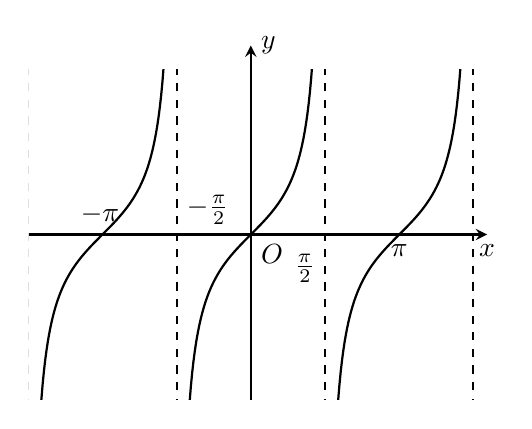
\begin{tikzpicture}[thick,>=stealth,scale=0.6]
		\draw[->] (-4.7,0) -- (5,0) node[below] {$x$};
		\draw[->] (0,-3.5) -- (0,4) node[right] {$y$};
		\draw (0,0) node[below right] {$O$};
		\clip(-4.7,-3.5) rectangle (5,3.5);
		\draw[thick,samples=100,domain=-1.325:1.36] plot(\x,{tan((\x)*180/pi)});
		\draw (-3.19,0) node[above] {$-\pi$};
		\draw (3.14,0) node[below] {$\pi$};
		\draw (-1.57,0) node[above right] {$-\frac{\pi}{2}$};
		\draw (1.57,-0.2) node[below left=-0.1] {$\frac{\pi}{2}$};
		\draw[dashed] (1.57,-4)--(1.57,5);
		\draw[dashed] (-1.57,-4)--(-1.57,5);
		\draw[dashed] (-4.71,-4)--(-4.71,5);
		\draw[dashed] (4.71,-4)--(4.71,5);
		\draw[thick,samples=100,domain=1.82:4.5] plot(\x,{tan((\x)*180/pi)});
		\draw[thick,samples=100,domain=-4.46:-1.79] plot(\x,{tan((\x)*180/pi)});
	\end{tikzpicture}
}
\begin{itemize}
	\item Hàm số $y=\tan x$ \fbox{đồng biến} trên mỗi khoảng $\left(-\dfrac{\pi}{2}+k \pi ; \dfrac{\pi}{2}+k \pi\right)$ với $k \in \mathbb{Z}$.
\end{itemize}
\subsubsection{Hàm số \boldmath$y=\cot x$\unboldmath}

\begin{itemize}
	\immini{\item  Điều kiện $\sin x \ne 0 \Leftrightarrow x \ne k\pi, k\in \mathbb{Z}$.\\
	      Tập xác định: \fbox{$\mathscr{D}=\mathbb{R}\setminus \left\{k\pi, k\in \mathbb{Z}\right\}.$}
	\item  \fbox{Tập giá trị: $\mathbb{R}.$}
	\item  Là \fbox{hàm số lẻ}
	\item \fbox{ĐTHS nhận gốc tọa độ $O$ làm tâm đối xứng}.
	\item  Là hàm số tuần hoàn với \fbox{chu kì $T=\pi$}, nghĩa là  $\cot(x+k\pi)=\cot x$, với $k \in \mathbb{Z}$.
	\item Hàm số $y=\cot x$ \fbox{nghịch biến} trên mỗi khoảng $(k \pi ; \pi+k \pi)$ với $k \in \mathbb{Z}$.
	      }{
	      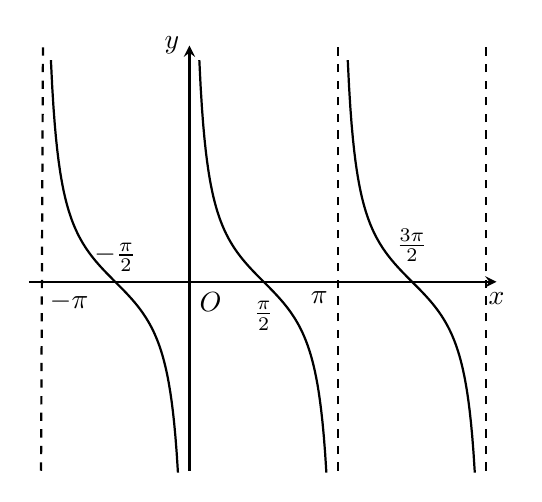
\begin{tikzpicture}[thick,>=stealth,scale=0.6]
		      \draw[->] (-3.4,0) -- (6.5,0) node[below] {$x$};
		      \draw[->] (0,-4) -- (0,5) node[left] {$y$};
		      \draw (0,0) node[below right] {$O$};
		      \draw[thick,samples=100,domain=0.21:2.9] plot(\x,{cot((\x)*180/pi)});
		      \draw[thick,samples=100,domain=0.21:2.9] plot(\x-pi,{cot((\x)*180/pi)});
		      \draw[thick,samples=100,domain=0.21:2.9] plot(\x+pi,{cot((\x)*180/pi)});
		      %\draw[thick,samples=100,domain=0.21:2.9] plot(\x-2*pi,{cot((\x)*180/pi)});
		      \draw (-3.17,0) node[below right] {$-\pi$};
		      \draw (3.14,0) node[below left=-0.1] {$\pi$};
		      \draw (-1.57,0) node[above] {$-\frac{\pi}{2}$};
		      \draw (1.57,-0.2) node[below] {$\frac{\pi}{2}$};
		      %\draw (-4.71,-0.2) node[below] {$-\frac{3\pi}{2}$};
		      \draw (4.71,0.2) node[above] {$\frac{3\pi}{2}$};
		      \draw[dashed] (3.14,-4)--(3.14,5);
		      \draw[dashed] (-3.14,-4)--(-3.1,5);
		      \draw[dashed] (6.28,-4)--(6.28,5);
		      %\draw[dashed] (-6.28,-4)--(-6.28,5);
	      \end{tikzpicture}}
\end{itemize}

\subsection{PHÂN LOẠI, PHƯƠNG PHÁP GIẢI TOÁN}

\begin{dang}{Tìm tập xác định của hàm số lượng giác}
	Ta chú ý một số điều kiện sau:
	\begin{enumerate}
		\item $y=\dfrac{f(x)}{g(x)}$ xác định $ \Leftrightarrow g(x)\ne 0$.
		\item $y=\sqrt[2n]{f(x)}$ xác định $ \Leftrightarrow f(x)\geqslant 0$, trong đó $n\in \mathbb{N}^*$.
		\item $y=\tan \left[u(x)\right]$ xác định $ \Leftrightarrow u(x)$ xác định và $u(x)\ne \dfrac{\pi}{2}+k\pi,k\in \mathbb{Z}$.
		\item $y=\cot \left[u(x)\right]$ xác định $ \Leftrightarrow u(x)$ xác định và $u(x)\ne k\pi,k\in \mathbb{Z}$.
	\end{enumerate}
\end{dang}

\begin{vd}
	Tìm tập xác định của các hàm số sau đây:
	\begin{tasks}(1)
		\task $y=\dfrac{2\sin x+3}{\cos x}$ \dotfill
		\task $y=\dfrac{1+\cos x}{1-\cos x}$\dotfill
		\task $y=\dfrac{\sin x-3}{\cos x+1}$ \dotfill
		\task $y=\dfrac{2+3\cos 2x}{\sin x}$ \dotfill
		\task $y=\dfrac{1+\cos x}{1+\sin x}$\dotfill
		\task $y=\dfrac{2\sin x+3}{\sin x-1}$ \dotfill
		\task $y=\dfrac{2\sin x-3}{2\sin x+3}$ \dotfill
		\task $y=\dfrac{2\sin x+3}{\cos x+2}$ \dotfill
		\task $y=\sqrt{3-2\cos x}$\dotfill
	\end{tasks}
	\loigiai{
		\begin{enumerate}[a)]
			\item Hàm số xác định khi $\cos x \ne 0 \Leftrightarrow x \ne \dfrac{\pi}{2} + k\pi$ ($k \in \mathbb{Z}$).\\
			      Vậy $\mathscr{D} = \mathbb{R} \setminus \left\{\dfrac{\pi}{2} + k\pi, k \in \mathbb{Z}\right\}$.

			\item Hàm số xác định khi $1 - \cos x \ne 0 \Leftrightarrow \cos x \ne 1 \Leftrightarrow x \ne k2\pi$ ($k \in \mathbb{Z}$).\\
			      Vậy $\mathscr{D} = \mathbb{R} \setminus \{k2\pi, k \in \mathbb{Z}\}$.

			\item Hàm số xác định khi $\cos x + 1 \ne 0 \Leftrightarrow \cos x \ne -1 \Leftrightarrow x \ne \pi + k2\pi$ ($k \in \mathbb{Z}$).\\
			      Vậy $\mathscr{D} = \mathbb{R} \setminus \{\pi + k2\pi, k \in \mathbb{Z}\}$.

			\item Hàm số xác định khi $\sin x \ne 0 \Leftrightarrow x \ne k\pi$ ($k \in \mathbb{Z}$).\\
			      Vậy $\mathscr{D} = \mathbb{R} \setminus \{k\pi, k \in \mathbb{Z}\}$.

			\item Hàm số xác định khi $1 + \sin x \ne 0 \Leftrightarrow \sin x \ne -1 \Leftrightarrow x \ne -\dfrac{\pi}{2} + k2\pi$ ($k \in \mathbb{Z}$).\\
			      Vậy $\mathscr{D} = \mathbb{R} \setminus \left\{-\dfrac{\pi}{2} + k2\pi, k \in \mathbb{Z}\right\}$.

			\item Hàm số xác định khi $\sin x - 1 \ne 0 \Leftrightarrow \sin x \ne 1 \Leftrightarrow x \ne \dfrac{\pi}{2} + k2\pi$ ($k \in \mathbb{Z}$).\\
			      Vậy $\mathscr{D} = \mathbb{R} \setminus \left\{\dfrac{\pi}{2} + k2\pi, k \in \mathbb{Z}\right\}$.

			\item Hàm số xác định khi $2\sin x + 3 \ne 0 \Leftrightarrow \sin x \ne -\dfrac{3}{2}$ (luôn đúng vì $-1 \le \sin x \le 1$).\\
			      Vậy $\mathscr{D} = \mathbb{R}$.

			\item Hàm số xác định khi $\cos x + 2 \ne 0 \Leftrightarrow \cos x \ne -2$ (luôn đúng vì $-1 \le \cos x \le 1$).\\
			      Vậy $\mathscr{D} = \mathbb{R}$.

			\item Hàm số xác định khi $3 - 2\cos x \ge 0 \Leftrightarrow \cos x \le \dfrac{3}{2}$ (luôn đúng vì $-1 \le \cos x \le 1$).\\
			      Vậy $\mathscr{D} = \mathbb{R}$.
		\end{enumerate}
	}
\end{vd} \dongcham{32}
\begin{vd}
	Tìm tập xác định của các hàm số sau đây:
	\begin{tasks}(1)
		\task $y=2\tan x+3$ \dotfill
		\task $y=2\tan 2x-4\sin x$\dotfill\\
		.\dotfill
		\task $y=\cot \left(x+\dfrac{\pi}{4} \right)+1$ \dotfill
	\end{tasks}
	\loigiai{
		\begin{enumerate}[a)]
			\item Hàm số xác định khi $\cos x \ne 0 \Leftrightarrow x \ne \dfrac{\pi}{2} + k\pi$ ($k \in \mathbb{Z}$).\\
			      Vậy tập xác định là $\mathscr{D} = \mathbb{R} \setminus \left\{\dfrac{\pi}{2} + k\pi, k \in \mathbb{Z}\right\}$.

			\item Hàm số xác định khi $\cos 2x \ne 0 \Leftrightarrow 2x \ne \dfrac{\pi}{2} + k\pi \Leftrightarrow x \ne \dfrac{\pi}{4} + k\dfrac{\pi}{2}$ ($k \in \mathbb{Z}$).\\
			      Vậy tập xác định là $\mathscr{D} = \mathbb{R} \setminus \left\{\dfrac{\pi}{4} + k\dfrac{\pi}{2}, k \in \mathbb{Z}\right\}$.

			\item Hàm số xác định khi $\sin\left(x + \dfrac{\pi}{4}\right) \ne 0 \Leftrightarrow x + \dfrac{\pi}{4} \ne k\pi \Leftrightarrow x \ne -\dfrac{\pi}{4} + k\pi$ ($k \in \mathbb{Z}$).\\
			      Vậy tập xác định là $\mathscr{D} = \mathbb{R} \setminus \left\{-\dfrac{\pi}{4} + k\pi, k \in \mathbb{Z}\right\}$.
		\end{enumerate}
	}
\end{vd} \dongcham{15}

\begin{dang}{Tính chẵn lẻ của hàm số}
	Ta thực hiện các bước sau:
	\begin{enumerate}
		\item[\ding{172}] Tìm tập xác định $\mathscr{D}$ của hàm số -- Tập $\mathscr{D}$ phải đối xứng.
		\item[\ding{173}] Tính $f\left(-x\right)$ (\textit{chỗ nào có biến $x$, ta thay bởi $-x$}) và thu gọn kết quả. Khi đó
		      \begin{itemize}
			      \item [$\bullet$] Nếu $f(-x)=f(x)$: hàm số đã cho là hàm chẵn.
			      \item [$\bullet$] Nếu $f(-x)=-f(x)$: hàm số đã cho là hàm lẻ.
			      \item [$\bullet$] Nếu không rơi vào 2 trường hợp trên, ta kết luận hàm số không chẵn, không lẻ.
		      \end{itemize}
	\end{enumerate}

	\begin{khung4}{GHI NHỚ}
		\begin{listEX}[1]
			\item [\ding{172}] Hàm số $y=\sin x$, $y=\tan x$, $y=\cot x$ là hàm số lẻ.
			\item [\ding{173}] Hàm số $y=\cos x$ là hàm số chẵn.
		\end{listEX}
	\end{khung4}
\end{dang}

\begin{vd} Xét tính chẵn, lẻ của các hàm số:
	\begin{tasks}(1)
		\task $y=\sin x\cdot\cos x$\dotfill
		\task $y=\tan x+\cot x$\dotfill
		\task $y=\sin^2x$\dotfill
		\task $y=|\sin x | \cos x$ \dotfill
	\end{tasks}
	\loigiai{
		\hfill
		\begin{enumerate}[a)]
			\item Hàm số $y=f(x)=\sin x\cdot\cos x$ là hàm số lẻ vì:
			      \begin{itemize}
				      \item Tập xác định là $D=\mathbb{R}$.
				      \item $\forall x\in \mathbb{R}$ thì $-x\in\mathbb{R}$ và $f\left(-x\right)=\sin\left(-x\right)\cdot\cos\left(-x\right)=-\left(\sin x\cdot\cos x\right)=-f(x)$.
			      \end{itemize}
			\item Hàm số $y=g(x)=\tan x+\cot x$ là hàm số lẻ vì:
			      \begin{itemize}
				      \item Tập xác định là $D=\mathbb{R}\setminus\left\{\dfrac{\pi}{2}\big|k\in\mathbb{Z}\right\}$.
				      \item $\forall x\in \mathbb{R}$ thì $-x\in D$ và $g\left(-x\right)=\tan\left(-x\right)+\cot\left(-x\right)=-\left(\tan x+\cot x\right)=-g(x)$.
			      \end{itemize}
			\item Hàm số $y=h(x)=\sin^2x$ là hàm số chẵn vì:
			      \begin{itemize}
				      \item Tập xác định là $D=\mathbb{R}$.
				      \item $\forall x\in \mathbb{R}$ thì $-x\in\mathbb{R}$ và $h\left(-x\right)=\sin^2\left(-x\right)=\left(-\sin x\right)^2=\sin^2x=h(x)$.
			      \end{itemize}
			\item Hàm số $y=f(x)=|\sin x | \cos x$ là hàm số chẵn vì:
			      \begin{itemize}
				      \item Tập xác định là $D=\mathbb{R}$.
				      \item $\forall x\in \mathbb{R}$ thì $-x\in\mathbb{R}$ và $f\left(-x\right)=|\sin (-x) | \cos (-x)=|-\sin x | \cos x=|\sin x | \cos x=f(x)$.
			      \end{itemize}
		\end{enumerate}
	}
\end{vd}
\dongcham{10}
\begin{dang}{Tìm chu kỳ của hàm số lượng giác}
	\begin{itemize}
		\item Hàm số $y=\sin x$, $y=\cos x$ tuần hoàn với chu kỳ $T_0=2\pi$, nghĩa là $\sin(x+k2\pi)=\sin x$ và $\cos(x+k2\pi)=\cos x$.\\
		      Suy ra hàm số $y=\sin(ax+b)$ và $y=\cos(ax+b)$ tuần hoàn với chu kỳ $T_0=\dfrac{2\pi}{|a|}$.
		\item Hàm số $y=\tan x$, $y=\cot x$ tuần hoàn với chu kỳ $T_0=\pi$.\\
		      Suy ra hàm số $y=\tan(ax+b)$ và $y=\cot(ax+b)$ tuần hoàn với chu kỳ $T_0=\dfrac{\pi}{|a|}$.
	\end{itemize}
	\begin{note}
		Giả sử hàm số $f(x)=g(x)\pm h(x)$ có hàm $g(x)$ tuần hoàn với chu kỳ $T_1$ và hàm $h(x)$ tuần hoàn với chu kỳ $T_2$. Khi đó hàm số $f(x)$ sẽ tuần hoàn với chu kỳ $T_0$ là bội chung nhỏ nhất của hai chu kỳ $T_1$ và $T_2$.
	\end{note}
\end{dang}
\setcounter{ex}{0}
\Opensolutionfile{ans}[ans/ans-1K1-3-dang4]
\begin{ex}%[THPT Kinh Môn 2 $-$ Hải Dương]%[Danh Trần - DA2.1]%[1D1Y1-4]
	Hàm số $y=\sin 2x$ tuần hoàn với chu kỳ chu kỳ là
	\choice
	{$T_0=2\pi$}
	{$T_0=\dfrac{\pi}{2}$}
	{\True $T_0=\pi$}
	{$T_0=4\pi$}
	\loigiai
	{
		Ta có hàm số $y=\sin 2x$ tuần hoàn với chu kỳ $T_0=\dfrac{2\pi}{2}=\pi$.
	}
\end{ex}
\begin{ex}%[THPT Thạch Thành $-$ Thanh Hóa]%[Danh Trần - DA2.1]%[1D1Y1-4]
	Hàm số $y=\tan 2x$ tuần hoàn với chu kỳ chu kỳ là
	\choice
	{$T_0=\dfrac{\pi}{3}$}
	{\True $T_0=\dfrac{\pi}{2}$}
	{$T_0=2\pi$}
	{$T_0=\pi$}
	\loigiai
	{
		Ta có hàm số $y=\tan 2x$ tuần hoàn với chu kỳ $T=\dfrac{\pi}{2}$.
	}
\end{ex}
\begin{ex}%[THPT Xuân Hòa $-$ Nam Định]%[Danh Trần - DA2.1]%[1D1B1-4]
	Hàm số $y=3\sin\dfrac{x}{2}$ tuần hoàn với chu kỳ chu kỳ là
	\choice
	{$T_0=0$}
	{$T_0=\dfrac{\pi}{2}$}
	{$T_0=2\pi$}
	{\True $T_0=4\pi$}
	\loigiai
	{
		Ta có hàm số $y=3\sin\dfrac{x}{2}$ tuần hoàn với chu kỳ $T=\dfrac{2\pi}{\tfrac{1}{2}}=4\pi$.
	}
\end{ex}
\begin{ex}%[THPT chuyên Hạ Long $-$ Quảng Ninh]%[Danh Trần - DA2.1]%[1D1K1-4]
	Hàm số $f(x)=\sin\dfrac{x}{2}+2\cos\dfrac{3x}{2}$ tuần hoàn với chu kỳ chu kỳ là
	\choice
	{$5\pi$}
	{$\dfrac{\pi}{2}$}
	{$3\pi$}
	{\True $4\pi$}
	\loigiai
	{
		Ta có hàm số $\sin\dfrac{x}{2}$ tuần hoàn với chu kỳ $T_1=\dfrac{2\pi}{\tfrac{1}{2}}=4\pi$, hàm số $\cos\dfrac{3x}{2}$ tuần hoàn với chu kỳ $T_2=\dfrac{2\pi}{\tfrac{3}{2}}=\dfrac{4\pi}{3}$.\\
		Do đó hàm số $f(x)$ tuần hoàn với chu kỳ $T_0$ là bội chung nhỏ nhất của $T_1$ và $T_2$.\\
		Do $T_1$ là bội của $T_2$ $\left(\dfrac{T_1}{T_2}=3\right)$ nên $T_0=T_1$.\\
		Vậy hàm số $f(x)$ đã cho tuần hoàn với chu kỳ $T_0=4\pi$.
	}
\end{ex}
\begin{ex}%[THPT Lê Trọng Tấn $-$ Tp. HCM]%[Danh Trần - DA2.1]%[1D1B1-4]
	Tìm $m$ để hàm số $y=\cos mx$ tuần hoàn với chu kỳ $T_0=\pi$.
	\choice
	{$m=\pm1$}
	{\True $m=\pm2$}
	{$m=\pm\dfrac{\pi}{2}$}
	{$m=\pm\pi$}
	\loigiai
	{
		Ta có hàm số $y=\cos mx$ tuần hoàn với chu kỳ $T=\dfrac{2\pi}{|m|}$.\\
		Để hàm số tuần hoàn với chu kỳ $T_0=\pi$ thì $T=T_0\Leftrightarrow \dfrac{2\pi}{|m|}=\pi\Leftrightarrow |m|=2\Leftrightarrow m=\pm2$.
	}
\end{ex}
\Closesolutionfile{ans}
\begin{dang}{Tìm giá trị lớn nhất - giá trị nhỏ nhất, tập giá trị của hàm số}
	Ta thường dùng một trong 3 phương pháp sau:
	\begin{enumerate}[\faCheckSquareO]
		\item Sử dụng các bất đẳng thức cơ bản
		      \begin{listEX}[2]
			      \item [\ding{172}] $-1 \leq \sin x \leq 1,\forall x \in \mathbb{R}$;
			      \item [\ding{173}] $-1 \leq \cos x \leq 1,\forall x\in \mathbb{R}$;
			      \item [\ding{174}] $0 \leq \sin^2x, \cos^2 x\leq 1,\forall x \in \mathbb{R}$;
			      \item [\ding{175}]  $0 \leq |\sin x|, |\cos x| \leq 1,\forall x \in \mathbb{R}$.
		      \end{listEX}
		      % \item Sử dụng điều kiện có nghiệm
		      % \begin{listEX}[1]
		      % 	\item [\ding{172}] $\sin x = f(m)$ có nghiệm khi $-1\le f(m) \le 1$.
		      % 	\item [\ding{173}] $\cos x = f(m)$ có nghiệm khi $-1\le f(m) \le 1$.
		      % 	\item [\ding{174}] $a\sin x + b\cos x = c$ có nghiệm khi $a^2+b^2 \ge c^2$.
		      % \end{listEX}
		\item Sử dụng bảng biến thiên: Lập bảng biến thiên của hàm số, từ đó, kết luận.
	\end{enumerate}
\end{dang}

\begin{vd}
	Tìm tập giá trị của các hàm số sau
	\begin{tasks}(1)
		\task $y=2\sin x+3$\dotfill
		\task $y=\dfrac{1-2{{\sin}^2}x}{3}$ \dotfill
		\task $y=\sqrt{2+\cos x}-1$ \dotfill
		\task $y=4\sin x\cos x+1$\dotfill
		\task $y=4-3\sin^22x$\dotfill
		\task $y={\left(3-\sin x \right)^2}+1$ \dotfill
	\end{tasks}
	\loigiai{
		\begin{enumerate}[a)]
			\item Ta có $-1 \le \sin x \le 1$ với mọi $x \in \mathbb{R}$\\
			      $\Rightarrow -2 \le 2\sin x \le 2 \Rightarrow 1 \le 2\sin x + 3 \le 5$.\\
			      Do đó $\min y = 1$ khi $\sin x = -1 \Leftrightarrow x = -\dfrac{\pi}{2} + k2\pi$ ($k \in \mathbb{Z}$).\\
			      $\max y = 5$ khi $\sin x = 1 \Leftrightarrow x = \dfrac{\pi}{2} + k2\pi$ ($k \in \mathbb{Z}$).\\
			      Vậy hàm số đã cho có tập giá trị $[1;5]$.

			\item Ta có $y = \dfrac{1 - 2\sin^2 x}{3} = \dfrac{\cos 2x}{3}$.\\
			      Vì $-1 \le \cos 2x \le 1$ với mọi $x \in \mathbb{R} \Rightarrow -\dfrac{1}{3} \le \dfrac{\cos 2x}{3} \le \dfrac{1}{3}$.\\
			      Do đó $\min y = -\dfrac{1}{3}$ khi $\cos 2x = -1 \Leftrightarrow 2x = \pi + k2\pi \Leftrightarrow x = \dfrac{\pi}{2} + k\pi$ ($k \in \mathbb{Z}$).\\
			      $\max y = \dfrac{1}{3}$ khi $\cos 2x = 1 \Leftrightarrow 2x = k2\pi \Leftrightarrow x = k\pi$ ($k \in \mathbb{Z}$).\\
			      Vậy hàm số đã cho có tập giá trị $\left[-\dfrac{1}{3};\dfrac{1}{3}\right]$.

			\item Ta có $-1 \le \cos x \le 1$ với mọi $x \in \mathbb{R} \Rightarrow 1 \le 2 + \cos x \le 3$\\
			      $\Rightarrow 1 \le \sqrt{2 + \cos x} \le \sqrt{3} \Rightarrow 0 \le \sqrt{2 + \cos x} - 1 \le \sqrt{3} - 1$.\\
			      Do đó $\min y = 0$ khi $\cos x = -1 \Leftrightarrow x = \pi + k2\pi$ ($k \in \mathbb{Z}$).\\
			      $\max y = \sqrt{3} - 1$ khi $\cos x = 1 \Leftrightarrow x = k2\pi$ ($k \in \mathbb{Z}$).\\
			      Vậy hàm số đã cho có tập giá trị $\left[0;\sqrt{3}-1\right]$.


			\item Ta có $y = 4\sin x\cos x + 1 = 2(2\sin x\cos x) + 1 = 2\sin 2x + 1$.\\
			      Vì $-1 \le \sin 2x \le 1$ với mọi $x \in \mathbb{R} \Rightarrow -2 \le 2\sin 2x \le 2 \Rightarrow -1 \le 2\sin 2x + 1 \le 3$.\\
			      Do đó $\min y = -1$ khi $\sin 2x = -1 \Leftrightarrow 2x = -\dfrac{\pi}{2} + k2\pi \Leftrightarrow x = -\dfrac{\pi}{4} + k\pi$ ($k \in \mathbb{Z}$).\\
			      $\max y = 3$ khi $\sin 2x = 1 \Leftrightarrow 2x = \dfrac{\pi}{2} + k2\pi \Leftrightarrow x = \dfrac{\pi}{4} + k\pi$ ($k \in \mathbb{Z}$).\\
			      Vậy hàm số đã cho có tập giá trị $\left[-1;3\right]$.


			\item Ta có $0 \le \sin^2 2x \le 1$ với mọi $x \in \mathbb{R}$\\
			      $\Rightarrow -3 \le -3\sin^2 2x \le 0 \Rightarrow 1 \le 4 - 3\sin^2 2x \le 4$.\\
			      Do đó $\min y = 1$ khi $\sin^2 2x = 1 \Leftrightarrow \cos 2x = 0 \Leftrightarrow 2x = \dfrac{\pi}{2} + k\pi \Leftrightarrow x = \dfrac{\pi}{4} + k\dfrac{\pi}{2}$ ($k \in \mathbb{Z}$).\\
			      $\max y = 4$ khi $\sin^2 2x = 0 \Leftrightarrow \sin 2x = 0 \Leftrightarrow 2x = k\pi \Leftrightarrow x = k\dfrac{\pi}{2}$ ($k \in \mathbb{Z}$).\\
			      Vậy hàm số đã cho có tập giá trị $\left[1;4\right]$.

			\item Ta có $-1 \le \sin x \le 1$ với mọi $x \in \mathbb{R} \Rightarrow -1 \le -\sin x \le 1 \Rightarrow 2 \le 3 - \sin x \le 4$\\
			      $\Rightarrow 4 \le (3 - \sin x)^2 \le 16 \Rightarrow 5 \le (3 - \sin x)^2 + 1 \le 17$.\\
			      Do đó $\min y = 5$ khi $3 - \sin x = 2 \Leftrightarrow \sin x = 1 \Leftrightarrow x = \dfrac{\pi}{2} + k2\pi$ ($k \in \mathbb{Z}$).\\
			      $\max y = 17$ khi $3 - \sin x = 4 \Leftrightarrow \sin x = -1 \Leftrightarrow x = -\dfrac{\pi}{2} + k2\pi$ ($k \in \mathbb{Z}$).\\
			      Vậy hàm số đã cho có tập giá trị $\left[5;17\right]$.
		\end{enumerate}
	}
\end{vd} \dongcham{20}
\begin{vd}
	Tìm $x$ để hàm số $y={\left(\sin x+3 \right)^2}-1$ đạt giá trị nhỏ nhất.
	\loigiai{
		Ta có $-1 \le \sin x \le 1$ với mọi $x \in \mathbb{R}$.
		Suy ra $2 \le \sin x + 3 \le 4$ với mọi $x \in \mathbb{R}$.
		Do đó $4 \le (\sin x + 3)^2 \le 16 \Rightarrow 3 \le (\sin x + 3)^2 - 1 \le 15$.

		Hàm số đạt giá trị nhỏ nhất bằng $3$ khi $\sin x + 3 = 2 \Leftrightarrow \sin x = -1 \Leftrightarrow x = -\dfrac{\pi}{2} + k2\pi$ ($k \in \mathbb{Z}$).
		Vậy $x = -\dfrac{\pi}{2} + k2\pi$ ($k \in \mathbb{Z}$) thì hàm số đạt giá trị nhỏ nhất.
	}
\end{vd} \dongcham{6}

\begin{vd}
	Tìm $x$ để hàm số $y=1-3\sqrt{1-{{\cos}^2}x}$ đạt giá trị nhỏ nhất.
	\loigiai{
		Ta có $-1 \le \cos x \le 1$ với mọi $x \in \mathbb{R} \Rightarrow 0 \le \cos^2 x \le 1 \Rightarrow 0 \le 1 - \cos^2 x \le 1$.
		Suy ra $0 \le \sqrt{1 - \cos^2 x} \le 1 \Rightarrow -3 \le -3\sqrt{1 - \cos^2 x} \le 0$.
		Do đó $-2 \le 1 - 3\sqrt{1 - \cos^2 x} \le 1$.

		Hàm số đạt giá trị nhỏ nhất bằng $-2$ khi $\sqrt{1 - \cos^2 x} = 1 \Leftrightarrow 1 - \cos^2 x = 1 \Leftrightarrow \cos^2 x = 0 \Leftrightarrow \cos x = 0 \Leftrightarrow x = \dfrac{\pi}{2} + k\pi$ ($k \in \mathbb{Z}$).
		Vậy $x = \dfrac{\pi}{2} + k\pi$ ($k \in \mathbb{Z}$) thì hàm số đạt giá trị nhỏ nhất.
	}
\end{vd} \dongcham{6}

\begin{vd}
	Tìm giá trị lớn nhất và nhỏ nhất của hàm số sau
	\begin{tasks}(1)
		\task $y=2{{\sin}^2}x-3\sin x+1$\dotfill
		\task $y=2{{\cos}^2}x+3\cos x-2$\dotfill
		\task  $y=\cos 2x-\sin x+3$\dotfill
	\end{tasks}
	\loigiai{
		\begin{enumerate}[a)]
			\item Đặt $t = \sin x$, với $x \in \mathbb{R}$ thì $t \in [-1; 1]$.
			      Hàm số trở thành $y = f(t) = 2t^2 - 3t + 1$ xét trên đoạn $[-1; 1]$.
			      Đồ thị hàm số $f(t)$ là một parabol có hoành độ đỉnh $t = \dfrac{3}{4} \in [-1; 1]$ và bề lõm hướng lên.

			      Bảng biến thiên:
			      \begin{center}
				      
\begin{tikzpicture}
					      \tkzTabInit[lgt=1.2,espcl=2.5]
					      {$t$/.7, $f(t)$/2}
					      {$-1$, $\frac{3}{4}$, $1$}
					      \tkzTabVar{+/ $6$, -/ $-\dfrac{1}{8}$, +/ $0$}
				      \end{tikzpicture}
			      \end{center}

			      Dựa vào bảng biến thiên, ta có:
			      $\min y = -\dfrac{1}{8}$ khi $t = \dfrac{3}{4} \Leftrightarrow \sin x = \dfrac{3}{4}$.\\
			      $\max y = 6$ khi $t = -1 \Leftrightarrow \sin x = -1 \Leftrightarrow x = -\dfrac{\pi}{2} + k2\pi$ ($k \in \mathbb{Z}$).

			\item Đặt $t = \cos x$, với $x \in \mathbb{R}$ thì $t \in [-1; 1]$.
			      Hàm số trở thành $y = f(t) = 2t^2 + 3t - 2$ xét trên đoạn $[-1; 1]$.
			      Đồ thị hàm số $f(t)$ là một parabol có hoành độ đỉnh $t = -\dfrac{3}{4} \in [-1; 1]$ và bề lõm hướng lên.

			      Bảng biến thiên:
			      \begin{center}
				      
\begin{tikzpicture}
					      \tkzTabInit[lgt=1.2,espcl=2.5]
					      {$t$/.7, $f(t)$/2}
					      {$-1$, $-\frac{3}{4}$, $1$}
					      \tkzTabVar{+/ $-3$, -/ $-\dfrac{25}{8}$, +/ $3$}
				      \end{tikzpicture}
			      \end{center}

			      Dựa vào bảng biến thiên, ta có:
			      $\min y = -\dfrac{25}{8}$ khi $t = -\dfrac{3}{4} \Leftrightarrow \cos x = -\dfrac{3}{4}$.\\
			      $\max y = 3$ khi $t = 1 \Leftrightarrow \cos x = 1 \Leftrightarrow x = k2\pi$ ($k \in \mathbb{Z}$).

			\item Ta có $y = \cos 2x - \sin x + 3 = (1 - 2\sin^2 x) - \sin x + 3 = -2\sin^2 x - \sin x + 4$.
			      Đặt $t = \sin x$, với $x \in \mathbb{R}$ thì $t \in [-1; 1]$.
			      Hàm số trở thành $y = f(t) = -2t^2 - t + 4$ xét trên đoạn $[-1; 1]$.
			      Đồ thị hàm số $f(t)$ là một parabol có hoành độ đỉnh $t = -\dfrac{1}{4} \in [-1; 1]$ và bề lõm hướng xuống.

			      Bảng biến thiên:
			      \begin{center}
				      
\begin{tikzpicture}
					      \tkzTabInit[lgt=1.2,espcl=2.5]
					      {$t$/.7, $f(t)$/2}
					      {$-1$, $-\frac{1}{4}$, $1$}
					      \tkzTabVar{-/ $3$, +/ $\dfrac{33}{8}$, -/ $1$}
				      \end{tikzpicture}
			      \end{center}

			      Dựa vào bảng biến thiên, ta có:
			      $\min y = 1$ khi $t = 1 \Leftrightarrow \sin x = 1 \Leftrightarrow x = \dfrac{\pi}{2} + k2\pi$ ($k \in \mathbb{Z}$).\\
			      $\max y = \dfrac{33}{8}$ khi $t = -\dfrac{1}{4} \Leftrightarrow \sin x = -\dfrac{1}{4}$.
		\end{enumerate}
	}
\end{vd} \dongcham{19}
\begin{vd}%[Dự án BGK10-11,2024]%[Nguyễn Văn Nay]%[1D1C4-6] 	[Mức độ 4]
	Tìm giá trị lớn nhất và giá trị nhỏ nhất của các hàm số sau trên mỗi đoạn cho trước
	\begin{enumerate}
		\item $y=\sin \left(2 x+\dfrac{\pi}{4}\right)+\dfrac{1}{2}$ trên $\left[-\dfrac{\pi}{4} ; \dfrac{\pi}{4}\right]$.\dotfill
		\item $y=-\cos\left(2x+\dfrac{\pi}{3}\right)$ trên $\left[-\dfrac{2\pi}{3}; \dfrac{\pi}{3}\right]$.\dotfill
	\end{enumerate}
	\loigiai
	{\immini
		{Ta có $x\in \left[ -\dfrac{\pi}{4} ; \dfrac{\pi}{4}\right]\Rightarrow 2x+\dfrac{\pi}{4}\in \left[ -\dfrac{\pi}{4}; \dfrac{3\pi}{4}\right]$.\\
			Do đó:
			\allowdisplaybreaks
			\begin{eqnarray*}
				& & -\dfrac{\sqrt{2}}{2}\leq \sin \left(2 x+\dfrac{\pi}{4}\right)\leq 1\\
				&\Rightarrow & \dfrac{1-\sqrt{2}}{2}\leq \sin \left(2 x+\dfrac{\pi}{4}\right)+\dfrac{1}{2}\leq \dfrac{3}{2}.
			\end{eqnarray*}
			Vậy $\max\limits_{x \in\left[-\tfrac{\pi}{4} ; \tfrac{\pi}{4}\right]} y=\dfrac{3}{2}$ và $\min\limits_{x \in \left[-\tfrac{\pi}{4} ; \tfrac{\pi}{4}\right]} y=\dfrac{1-\sqrt{2}}{2}$.
		}
		{
			\begin{tikzpicture}[line join=round, line cap=round,>=stealth,thick,scale=1.4]
				\tikzset{label style/.style={font=\footnotesize}}
				\draw[->] (-1.2,0)--(1.4,0) node[below] {$x$};
				\draw[->] (0,-1.2)--(0,1.3) node[left] {$y$};
				\draw (0,0) circle (1);
				\draw (0,0) node [below left] {$O$};
				\path
				(0,0) coordinate (O)
				($(O) + (-45:1.1)$) coordinate (A)
				($(O) + (135:1.1)$) coordinate (B)
				;
				\draw[red,<->] (A) arc (-45:135:1.1 cm);
				\draw (O) -- (A) node [right] {\scriptsize $-\frac{\pi}{4}$};
				\draw (O) -- (B) node [left] {\scriptsize $\frac{3\pi}{4}$};
				\draw[dashed] (-45:1) -- (0,-0.7) node [left] {\scriptsize $-\frac{\sqrt{2}}{2}$};
				\draw[dashed] (135:1) -- (0,0.7) node [right] {\scriptsize $\frac{\sqrt{2}}{2}$};
			\end{tikzpicture}
		}
	}
\end{vd}
\begin{vd}
	\immini{Khi đu quay hoạt động, vận tốc theo phương ngang của một cabin $M$ phụ thuộc vào góc lượng giác $\alpha=(Ox, OM)$ theo hàm số $v_x=0,3\sin \alpha\,(\mathrm{m} / \mathrm{s})$ (Hình bên).
		\begin{tasks}
			\task Tìm giá trị lớn nhất và giá trị nhỏ nhất của $v_{x}$
			\task Dựa vào đồ thị của hàm số sin, hãy cho biết trong vòng quay đầu tiên $(0 \leq \alpha \leq 2 \pi)$, góc $\alpha$ ở trong các khoảng nào thì $v_x$ tăng.
		\end{tasks}}{
		\begin{tikzpicture}[scale=0.7,>=stealth]
			\def\r{3}
			\def\a{\r/10}
			\def\n{12}%Số nan đu quay
			\def\m{12}%Số lồng đu quay
			\pgfmathsetmacro{\g}{20}
			\pgfmathsetmacro{\b}{2*\a/3}
			\pgfmathsetmacro{\xo}{\a *cos(\g)}
			\pgfmathsetmacro{\yo}{\b *sin(\g)}
			\def\longdq(#1:#2){
				\begin{scope}[shift={(#1:#2)}]
					\draw (0,-\b) ellipse ({\b/2} and {\b});
					\fill[blue!60] (\xo,\yo-\b) arc (\g:-180-\g:{\a} and {\b})--cycle;
					\draw (0,-\b) ellipse({\a} and {\b});
				\end{scope}
			}
			\foreach \i in {1,...,\n}{
					\pgfmathsetmacro{\gm}{360*\i/\n}
					\pgfmathsetmacro{\gh}{(360*\i+180)/\n}
					\pgfmathsetmacro{\gb}{360*(\i+1)/\n}
					\draw (\gm:\r-\a)--(\gh:\r)--(\gb:\r-\a);
					\draw (\gm:\r-\a)--(\gm:\a);
				}
			\draw[double] (0:0) circle (\r);
			\draw (0:0) circle (\r-\a);
			\foreach \i in {1,...,\m}{\longdq(360*\i/\m:\r)}
			\draw[top color =gray!10, bottom color=gray!30] (-30:\a) arc(-30:0:\a) --(-70:1.5*\r)--++(\a/2,0)--([turn]-70:\r/2) --([turn]-110:3*\a)--(-30:\a);
			\draw[top color =gray!10, bottom color=gray!30, xscale=-1] (-30:\a) arc(-30:0:\a) --(-70:1.5*\r)--++(\a/2,0)--([turn]-70:\r/2) --([turn]-110:3*\a)--(-30:\a);
			\fill[ball color=orange] (0:0) circle (\a);
			\draw[double] (0:0) circle (\a);
			\draw[->] (-4,0)--(5,0) node[below]{$x$};
			\draw (0,0) node[above left]{$O$};
			\coordinate (O) at (0,0);
			\coordinate (A) at ($(O) + (0:3)$);
			\coordinate (M) at ($(O) + (30:3)$);
			\draw[thick,red] (A)--(O)--(M);
			\foreach \x/\g in {A/50,M/50}\draw[fill=black] (\x) circle (.05) +(\g:.5)node{\footnotesize$\x$};
			\draw [shift={(0,0)},line width=0.3pt] (0:.9) arc (0:15:.9) node[right]{\scriptsize$\alpha$};
			\draw [shift={(0,0)},->,line width=0.3pt] (0:.9) arc (0:30:.9);
			\coordinate (O') at ($(M)!0.75!-90:(O)$);
			\draw[->] (M)--(1.5,1.5)node[below left=-2pt]{\scriptsize$\vec{v}_x$};
			\draw[->] (M)--(O')node[above right=-1pt]{\scriptsize$\vec{v}$};
			\draw[dashed] (1.5,1.5)--(O');
			%\draw[dashed] (0,-5.66)--(5,-5.66)node[below]{\text{ Mặt đất}};
			%\draw[<->] (4,0)--(4,-5.66)node[pos=.5,right]{\footnotesize$h=13$ m};
			%\draw[<->] (4,0)--(4,3)node[pos=.5,right]{\footnotesize$R=10$ m};
		\end{tikzpicture}}
	\loigiai{
		\begin{enumerate}[a)]
			\item Ta có $-1 \le \sin \alpha \le 1$ với mọi $\alpha \in \mathbb{R}$.
			      Suy ra $-0{,}3 \le 0{,}3 \sin \alpha \le 0{,}3 \Rightarrow -0{,}3 \le v_x \le 0{,}3$.
			      Vậy giá trị lớn nhất của $v_x$ là $0{,}3$ m/s, đạt được khi $\sin \alpha = 1 \Leftrightarrow \alpha = \dfrac{\pi}{2} + k2\pi$ ($k \in \mathbb{Z}$).
			      Giá trị nhỏ nhất của $v_x$ là $-0{,}3$ m/s, đạt được khi $\sin \alpha = -1 \Leftrightarrow \alpha = -\dfrac{\pi}{2} + k2\pi$ ($k \in \mathbb{Z}$).

			\item Hàm số $v_x = 0{,}3 \sin \alpha$ tăng khi và chỉ khi hàm số $y = \sin \alpha$ đồng biến.
			      Dựa vào đồ thị của hàm số sin, trên đoạn $[0; 2\pi]$ (ứng với vòng quay đầu tiên), hàm số $y = \sin \alpha$ đồng biến trên các khoảng $\left(0; \dfrac{\pi}{2}\right)$ và $\left(\dfrac{3\pi}{2}; 2\pi\right)$.
			      Vậy trong vòng quay đầu tiên, góc $\alpha$ thuộc các khoảng $\left(0; \dfrac{\pi}{2}\right)$ và $\left(\dfrac{3\pi}{2}; 2\pi\right)$ thì vận tốc $v_x$ tăng.
		\end{enumerate}
	}
\end{vd} \dongcham{7}

\begin{dang}{Đồ thị hàm số lượng giác}
\end{dang}

\begin{vd} Xét sự biến thiên của mỗi hàm số sau trên các khoảng tương ứng:
	\begin{enumerate}[a)]
		\item 	$y=\sin x$ trên khoảng $\left(-\dfrac{9 \pi}{2} ;-\dfrac{7 \pi}{2}\right),\left(\dfrac{21 \pi}{2} ; \dfrac{23 \pi}{2}\right)$;
		\item 	$y=\cos x$ trên khoảng $(-20 \pi ;-19 \pi),(-9 \pi ;-8 \pi)$.
	\end{enumerate}
	\loigiai{
		\begin{enumerate}[a)]
			\item Ta có
			      \begin{itemize}
				      \item $\left( -\dfrac{9\pi }{2};-\dfrac{7\pi }{2} \right)=\,\left( -\dfrac{\pi }{2}-4\pi ;\dfrac{\pi }{2}-4\pi  \right)$.\\
				            Do hàm số $y=\sin x$ đồng biến trên khoảng $\left(-\dfrac{\pi}{2};\dfrac{\pi}{2}\right)$ nên hàm số đó cũng đồng biến trên khoảng $\left(-\dfrac{9\pi}{2};-\dfrac{7\pi}{2}\right)$.
				      \item $\left( \dfrac{21\pi }{2};\dfrac{23\pi }{2} \right)=\left( \dfrac{\pi }{2}+10\pi ;\dfrac{3\pi }{2}+10\pi  \right)$.\\
				            Do hàm số $y=\sin x$ nghịch biến trên khoảng $\left(\dfrac{\pi}{2};\dfrac{3\pi}{2}\right)$ nên hàm số đó cũng nghịch biến trên khoảng $\left(\dfrac{21\pi}{2};\dfrac{23\pi}{2}\right)$ .
			      \end{itemize}
			\item Ta có
			      \begin{itemize}
				      \item $\left( -20\pi ;-19\pi  \right)=\left( 0-20\pi ;\pi -20\pi  \right)$.\\
				            Do hàm số $y=\cos x$ nghịch biến trên khoảng $\left(0;\pi\right)$ nên hàm số đó cũng nghịch biến trên khoảng $\left(-20\pi ;-19\pi\right)$
				      \item $\left( -9\pi ;-8\pi  \right)=\left( -\pi -8\pi ;0-8\pi  \right)$.\\
				            Do hàm số $y=\cos x$ đồng biến trên khoảng $\left(-\pi ;0\right)$ nên hàm số đó cũng đồng biến trên khoảng $\left(-9\pi ;-8\pi\right)$
			      \end{itemize}
		\end{enumerate}
	}
\end{vd}
\dongcham{8}

\begin{vd} Xét sự biến thiên của mỗi hàm số sau trên các khoảng tương ứng:
	\begin{enumerate}[a)]
		\item 	$y=\sin 2x$ trên khoảng $\left(-\dfrac{9 \pi}{4} ;-\dfrac{7 \pi}{4}\right),\left(\dfrac{21 \pi}{4} ; \dfrac{23 \pi}{4}\right)$;
		\item 	$y=\cos \left( \dfrac23x-\dfrac{\pi}{4}\right) $ trên khoảng $\left( \dfrac{3\pi}{8};\dfrac{15\pi}{8}\right), \left( \dfrac{2031\pi}{8};\dfrac{2043\pi}{8}\right) $.
	\end{enumerate}
	\loigiai{
		\begin{enumerate}[a)]
			\item Xét $y=\sin 2x$. Đặt $t=2x$ (nhận xét: $t$ đồng biến theo biến $x$).
			      \begin{itemize}
				      \item Với $x \in \left(-\dfrac{9 \pi}{4} ;-\dfrac{7 \pi}{4}\right) \Rightarrow t \in \left(-\dfrac{9 \pi}{2} ;-\dfrac{7 \pi}{2}\right)=\left( -\dfrac{\pi}{2}-2\pi; \dfrac{\pi}{2}-2\pi\right)$.\\
				            Vì $\sin t$ đồng biến trên khoảng $\left( -\dfrac{\pi}{2}-2\pi; \dfrac{\pi}{2}-2\pi\right)$ nên $\sin 2x$ đồng biến trên $\left(-\dfrac{9 \pi}{4} ;-\dfrac{7 \pi}{4}\right)$.

				      \item Với $x \in \left(\dfrac{21 \pi}{4} ;\dfrac{23 \pi}{4}\right) \Rightarrow t \in \left(\dfrac{21 \pi}{2} ;\dfrac{23 \pi}{2}\right)=\left( \dfrac{\pi}{2}+10\pi; \dfrac{3\pi}{2}+10\pi\right)$.\\
				            Vì $\sin t$ nghịch biến trên khoảng $\left( \dfrac{\pi}{2}+10\pi; \dfrac{3\pi}{2}+10\pi\right)$ nên $\sin 2x$ nghịch biến trên $\left(\dfrac{21 \pi}{4} ;\dfrac{23 \pi}{4}\right)$.
			      \end{itemize}

			\item Xét $y=\cos \left(\dfrac{2}{3}x-\dfrac{\pi}{4}\right)$. Đặt $u=\dfrac{2}{3}x-\dfrac{\pi}{4}$ (nhận xét: $u$ đồng biến theo biến $x$).
			      \begin{itemize}
				      \item Với $x \in \left(\dfrac{3\pi}{8};\dfrac{15\pi}{8}\right) \Rightarrow u \in \left(\dfrac{2}{3} \cdot \dfrac{3\pi}{8}-\dfrac{\pi}{4}; \dfrac{2}{3} \cdot \dfrac{15\pi}{8}-\dfrac{\pi}{4}\right) = \left(\dfrac{\pi}{4}-\dfrac{\pi}{4}; \dfrac{5\pi}{4}-\dfrac{\pi}{4}\right) = (0; \pi)$.\\
				            Vì $\cos u$ nghịch biến trên khoảng $(0; \pi)$ nên $y$ nghịch biến trên $\left(\dfrac{3\pi}{8};\dfrac{15\pi}{8}\right)$.

				      \item Với $x \in \left(\dfrac{2031\pi}{8};\dfrac{2043\pi}{8}\right) \Rightarrow u \in \left(\dfrac{2}{3} \cdot \dfrac{2031\pi}{8}-\dfrac{\pi}{4}; \dfrac{2}{3} \cdot \dfrac{2043\pi}{8}-\dfrac{\pi}{4}\right) = \left(\dfrac{677\pi}{4}-\dfrac{\pi}{4}; \dfrac{681\pi}{4}-\dfrac{\pi}{4}\right) = (169\pi; 170\pi)$.\\
				            Vì $169\pi = 84 \cdot 2\pi + \pi \equiv \pi \pmod{2\pi}$ và $170\pi = 85 \cdot 2\pi \equiv 0 \pmod{2\pi}$, nên khoảng $(169\pi; 170\pi)$ tương ứng với $(\pi; 2\pi)$ (hay $(\pi; 0)$ khi viết theo một chu kỳ).\\
				            Hàm $\cos u$ đồng biến trên khoảng $(\pi; 2\pi)$ nên $y$ đồng biến trên $\left(\dfrac{2031\pi}{8};\dfrac{2043\pi}{8}\right)$.
			      \end{itemize}
		\end{enumerate}
	}
\end{vd}

\begin{vd} Một dao động điều hoà có phương trình li độ dao động là: $x=A\cos\left(\omega\,t+\varphi\right)$ , trong đó $t$ là thời gian tính bằng giây, $A$ là biên độ dao động và $x$ là li độ dao động đều được tính bằng centimét, $\omega >0$ . Khi đó, chu kì $T$ của dao động là $T=\dfrac{2\pi}{\omega}$ . Xác định giá trị của li độ khi $t=0,\,\,t=\dfrac{T}{4},\,\,t=\dfrac{T}{2},\,t=\dfrac{3T}{4},\,\,t=T$ và vẽ đồ thị biểu diễn li độ của dao động điều hoà trên đoạn $\left[0;2T\right]$ trong các trường hợp:
	\begin{tasks}(1)
		\task $A=3cm,\,\,\varphi=0$\dotfill\\
		.\dotfill\\
		.\dotfill\\
		.\dotfill\\
		.\dotfill\\
		\task $A=3cm,\,\,\varphi=-\dfrac{\pi}{2}$\dotfill\\
		.\dotfill\\
		.\dotfill\\
		.\dotfill\\
		.\dotfill\\
		\task $A=3cm,\,\,\varphi=\dfrac{\pi}{2}$\dotfill\\
		.\dotfill\\
		.\dotfill\\
		.\dotfill\\
		.\dotfill\\
	\end{tasks}
	\loigiai{
		%		\begin{figure}
		\begin{enumerate}[a)]
			\item Khi $A=3cm,\,\,\varphi=0$, ta có: $x=3\cos\left(\omega\,t\right)=3\cos\left(\dfrac{2\pi}{T}t\right)$.\\
			      \immini
			      {Ta có bảng xác định giá trị li độ tại một số thời điểm và đồ thị cần vẽ ở Hình 9:\\
				      \begin{tabular}{|c|c|c|c|c|c|}
					      \hline
					      $t$ & $0$ & $\dfrac{T}{4}$ & $\dfrac{T}{2}$ & $\dfrac{3T}{4}$ & $T$ \\
					      \hline
					      $x$ & $3$ & $0$            & $-3$           & $0$             & $3$ \\
					      \hline
				      \end{tabular}
			      }{
				      \begin{tikzpicture} [scale=0.6,>=stealth, font=\footnotesize, line join=round, line cap=round]
					      \draw[->] (0,0)--(4*pi+0.5,0) node[above] {$t$};
					      \draw[->] (0,-3.5)--(0,3.5) node[below left]{$x$};
					      \draw (0,0) node[below left]{$O$};
					      \def\xmin{0} \def\xmax{4*pi}
					      \draw[domain=\xmin:\xmax,samples=100, smooth] plot (\x, {3*cos(\x r)});
					      \draw[dashed] (\xmin,3)--(\xmax+0.5,3) (\xmin,-3)--(\xmax+0.5,-3);
					      \node at (0.5*pi,0) [below left]{$\dfrac{T}{4}$};
					      \node at (pi,0) [above]{$\dfrac{T}{2}$};
					      \node at (1.5*pi,0) [below right]{$\dfrac{3T}{4}$};
					      \node at (2*pi,0) [below]{$T$};
					      \node at (2.5*pi,0) [below left]{$\dfrac{5T}{4}$};
					      \node at (3*pi,0) [above]{$\dfrac{3T}{2}$};
					      \node at (3.5*pi,0) [below right]{$\dfrac{7T}{4}$};
					      \node at (4*pi,0) [below]{$2T$};
					      \draw[dashed] (pi,0)--(pi,-3);
					      \draw[dashed] (2*pi,0)--(2*pi,3);
					      \draw[dashed] (3*pi,0)--(3*pi,-3);
					      \draw[dashed] (4*pi,0)--(4*pi,3);
				      \end{tikzpicture}
				      %			\caption{}
			      }
			\item Khi $A=3cm,\,\,\varphi=-\dfrac{\pi}{2}$, ta có: $x=3\cos\left(\omega\,t-\dfrac{\pi}{2}\right)=3\cos\left(\dfrac{2\pi}{T}t-\dfrac{\pi}{2}\right)$.
			      \immini
			      {Ta có bảng xác định giá trị li độ tại một số thời điểm và đồ thị cần vẽ ở Hình 10:\\
				      \begin{tabular}{|c|c|c|c|c|c|}
					      \hline
					      $t$ & $0$ & $\dfrac{T}{4}$ & $\dfrac{T}{2}$ & $\dfrac{3T}{4}$ & $T$ \\
					      \hline
					      $x$ & $0$ & $3$            & $0$            & $-3$            & $0$ \\
					      \hline
				      \end{tabular}
			      }
			      {
				      \begin{tikzpicture} [scale=0.6,>=stealth, font=\footnotesize, line join=round, line cap=round]
					      \draw[->] (0,0)--(4*pi+0.5,0) node[above] {$t$};
					      \draw[->] (0,-3.5)--(0,3.5) node[below left]{$x$};
					      \draw (0,0) node[below left]{$O$};
					      \def\xmin{0} \def\xmax{4*pi}
					      \draw[domain=\xmin:\xmax,samples=100, smooth] plot (\x, {3*cos((\x-0.5*pi) r)});
					      \draw[dashed] (\xmin,3)--(\xmax+0.5,3) (\xmin,-3)--(\xmax+0.5,-3);
					      \node at (0.5*pi,0) [below left]{$\dfrac{T}{4}$};
					      \node at (pi,0) [below left]{$\dfrac{T}{2}$};
					      \node at (1.5*pi,0) [above]{$\dfrac{3T}{4}$};
					      \node at (2*pi,0) [below right]{$T$};
					      \node at (2.5*pi,0) [below]{$\dfrac{5T}{4}$};
					      \node at (3*pi,0) [below left]{$\dfrac{3T}{2}$};
					      \node at (3.5*pi,0) [above]{$\dfrac{7T}{4}$};
					      \node at (4*pi,0) [below right]{$2T$};
					      \draw[dashed] (0.5*pi,0)--(0.5*pi,3);
					      \draw[dashed] (1.5*pi,0)--(1.5*pi,-3);
					      \draw[dashed] (2.5*pi,0)--(2.5*pi,3);
					      \draw[dashed] (3.5*pi,0)--(3.5*pi,-3);
				      \end{tikzpicture}
				      %			\caption{}
			      }
			\item Khi $A=3cm,\,\,\varphi=\dfrac{\pi}{2}$, ta có: $x=3\cos\left(\omega\,t+\dfrac{\pi}{2}\right)=3\cos\left(\dfrac{2\pi}{T}t+\dfrac{\pi}{2}\right)$.
			      \immini
			      {Ta có bảng xác định giá trị li độ tại một số thời điểm và đồ thị cần vẽ ở Hình 11:\\
				      \begin{tabular}{|c|c|c|c|c|c|}
					      \hline
					      $t$ & $0$ & $\dfrac{T}{4}$ & $\dfrac{T}{2}$ & $\dfrac{3T}{4}$ & $T$ \\
					      \hline
					      $x$ & $0$ & $-3$           & $0$            & $3$             & $0$ \\
					      \hline
				      \end{tabular}
			      }
			      {
				      \begin{tikzpicture} [scale=0.6,>=stealth, font=\footnotesize, line join=round, line cap=round]
					      \draw[->] (0,0)--(4*pi+0.5,0) node[above] {$t$};
					      \draw[->] (0,-3.5)--(0,3.5) node[below left]{$x$};
					      \draw (0,0) node[below left]{$O$};
					      \def\xmin{0} \def\xmax{4*pi}
					      \draw[domain=\xmin:\xmax,samples=100, smooth] plot (\x, {3*cos((\x+0.5*pi) r)});
					      \draw[dashed] (\xmin,3)--(\xmax+0.5,3) (\xmin,-3)--(\xmax+0.5,-3);
					      \node at (0.5*pi,0) [above]{$\dfrac{T}{4}$};
					      \node at (pi,0) [below right]{$\dfrac{T}{2}$};
					      \node at (1.5*pi,0) [below]{$\dfrac{3T}{4}$};
					      \node at (2*pi,0) [below left]{$T$};
					      \node at (2.5*pi,0) [above]{$\dfrac{5T}{4}$};
					      \node at (3*pi,0) [below right]{$\dfrac{3T}{2}$};
					      \node at (3.5*pi,0) [below]{$\dfrac{7T}{4}$};
					      \node at (4*pi,0) [below]{$2T$};
					      \draw[dashed] (0.5*pi,0)--(0.5*pi,-3);
					      \draw[dashed] (1.5*pi,0)--(1.5*pi,3);
					      \draw[dashed] (2.5*pi,0)--(2.5*pi,-3);
					      \draw[dashed] (3.5*pi,0)--(3.5*pi,3);
				      \end{tikzpicture}
				      %			\caption{}
			      }
		\end{enumerate}
		%	\end{figure}
	}
\end{vd}
\dongcham{19}

\subsection{BÀI TẬP TỰ LUẬN}

\begin{bt}%[Mức độ 2]%[Dự án BG-K11-Lần-2]%[Ngô Quang Anh]%[1D1H4-2]
	Tìm tập xác định $\mathscr{D}$ của các hàm số sau
	\begin{tasks}(2)
		\task $y=3\tan^2\left(\dfrac{x}{2}-\dfrac{\pi}{4}\right).$
		\task $\mathscr{D} $ của hàm số $y=\dfrac{3\tan x - 5}{1-\sin^2 x}$.
		\task $y=\sqrt{\dfrac{2+\sin x}{1-\cos x}}$.
		\task $y=\cos 2x+\dfrac{1}{\tan x}+5$.
		\task $y=\dfrac{\cot x}{\cos x-1}$.
	\end{tasks}
	\loigiai{
		\begin{enumerate}[a)]
			\item Hàm số xác định $\Leftrightarrow \cos\left(\dfrac{x}{2}-\dfrac{\pi}{4}\right)\ne 0\Leftrightarrow \dfrac{x}{2}-\dfrac{\pi}{4}\ne \dfrac{\pi}{2}+k\pi \Leftrightarrow x\ne \dfrac{3\pi}{2}+k2\pi, k\in \mathbb{Z}.$\\
			      Vậy tập xác định $ \mathscr{D}=\mathbb{R}\setminus\left\{\dfrac{3\pi}{2}+k2\pi \,\middle|\, k\in \mathbb{Z}\right\}$.
			\item Hàm số xác định khi và chỉ khi $$\heva{&\cos x \ne 0 \\& 1-\sin^2 x \ne 0} \Leftrightarrow \cos x \ne 0 \Leftrightarrow x \ne \dfrac{\pi}{2}+k\pi,k\in \mathbb{Z} .$$
			      Vậy tập xác định của hàm số là $ \mathscr{D} =\mathbb{R} \setminus \left\{\dfrac{\pi}{2}+k\pi \,\middle|\, k\in \mathbb{Z} \right\}$.
			\item Hàm số xác định khi $\heva{&\dfrac{2+\sin x}{1-\cos x}\ge 0\\&1-\cos x\ne 0}\Leftrightarrow 1-\cos x\ne 0\Leftrightarrow \cos x\ne 1\Leftrightarrow x\ne k2\pi$, $k\in\mathbb{Z}$.\\
			      Vậy tập xác định $\mathscr{D}=\mathbb{R}\setminus \left\{k2\pi \mid k\in\mathbb{Z}\right\}$.
			\item Hàm số xác định khi $\heva{&\tan x\ne 0\\&\cos x\ne 0}\Leftrightarrow \heva{&x\ne k\pi\\&x\ne \dfrac{\pi}{2}+k\pi}\Leftrightarrow x\ne \dfrac{k\pi}{2}$ ($k\in \mathbb{Z}$).\\
			      Vậy tập xác định của hàm số là $\mathscr{D}=\mathbb{R}\setminus \left\{ \dfrac{k\pi}{2} \mid k\in \mathbb{Z} \right\}$.
			\item Hàm số xác định khi và chỉ khi $\heva{&\sin x\ne 0\\ &\cos x\ne 1}\Leftrightarrow\heva{&x\ne k\pi\\ &x\ne \ell2\pi}\ (k, \ell\in\mathbb{Z})\Leftrightarrow x\ne k\pi, k\in\mathbb{Z}$.\\
			      Vậy, tập xác định của hàm số $y=\dfrac{\cot x}{\cos x-1}$ là $\mathbb{R}\setminus\left\{k\pi \mid k\in\mathbb{Z}\right\}$.
		\end{enumerate}
	}
\end{bt}

\begin{bt}%[Bài giảng K10-11, Nguyễn Đắc Giáp]%[1D1H4-4][SBT Kết nối tri thức với cuộc sống - Mức độ 2]
	Xét tính chẵn lẻ của các  hàm số sau:
	\begin{enumEX}{2}
		\item $y=x \sin 3x$;
		\item  $y=\dfrac{1+\cos 3 x}{1-\cos 3x}$;
		\item  $y=x^3 \cos 2x$;
		\item  $y=\sin x-\cos x$.
	\end{enumEX}
	\loigiai{
		\begin{enumerate}
			\item Tập xác định của hàm số là $\mathscr{D}=\mathbb{R}$.\\
			      Nếu kí hiệu $f(x)=x \sin 3x$ thì với mọi $x \in \mathscr{D}$, ta có $-x \in \mathscr{D}$ và
			      $$	f(-x)=(-x) \sin (-3x)=x \sin 3 x=f(x).	$$
			      Vậy hàm số đã cho là hàm số chẵn.
			\item  Tập xác định của hàm số là $\mathscr{D}=\mathbb{R}\setminus \left\{k \dfrac{2 \pi}{3} \,\middle|\, k \in \mathbb{Z}\right\}$.\\
			      Nếu kí hiệu $f(x)=\dfrac{1+\cos 3x}{1-\cos 3x}$ thì với mọi $x \in \mathscr{D}$, ta có $-x \in \mathscr{D}$ và
			      $$f(-x)=\dfrac{1+\cos (-3x)}{1-\cos (-3x)}=\dfrac{1+\cos 3 x}{1-\cos 3 x}=f(x).$$
			      Vậy hàm số đã cho là hàm số chẵn.
			\item Tập xác định của hàm số là $\mathscr{D}=\mathbb{R}$.\\
			      Nếu kí hiệu $f(x)=x^3 \cos 2x$ thì với mọi $x \in \mathscr{D}$, ta có $-x \in \mathscr{D}$ và
			      $$f(-x)=(-x)^3 \cos (-2x)=-x^3 \cos 2x=-f(x).$$
			      Vậy hàm số đã cho là hàm số lẻ.
			\item Nếu kí hiệu $f(x)=\sin x-\cos x$
			      thì $f(-1)=\sin (-1)-\cos (-1)=-\sin 1-\cos 1 $ và $f(1)=\sin 1 -\cos 1$.\\
			      Vì $f(-1) \neq f(1)$ và $f(-1) \neq-f(1)$ nên hàm số đã cho không phải là hàm số chẵn, cũng không phải là hàm số lẻ.
		\end{enumerate}
	}
\end{bt}

\begin{bt}%[Dự án BGK10-11,2024]%[Nguyễn Văn Nay]%[1D1H4-6] 
	Tìm giá trị lớn nhất và giá trị nhỏ nhất của các hàm số sau
	\begin{tasks}(2)
		\task $ y=1-\dfrac{1}{2} \sin^2 2 x $.
		\task $ y=3-2|\sin 2 x| $.
		\task $ y=\sin x+\sin \left(x+{\dfrac{2\pi}{3}}\right)$.
		\task $y=\sqrt{3} \sin x-\cos x+5$.
		\task $y=4 \sin^2 x-4 \sin x+3$.
		\task $y=\cos^2 x-2 \cos x-4$.
		\task $y=\cos^4 x-2 \sin^2 x+1$.
		\task $y=\sin x+\cos x+2 \sin x \cos x-1$.
	\end{tasks}
	\loigiai{
		\begin{enumerate}[a)]
			\item $ y=1-\dfrac{1}{2} \sin^2 2 x $. \\
			      Tập xác định: $ \mathscr{D}=\mathbb{R}$. $ \forall x \in \mathbb{R} $, ta có
			      \begin{eqnarray*}
				      && 0 \leq  \sin^2 2 x \leq 1\\
				      &\Leftrightarrow& -\dfrac{1}{2} \leq  -\dfrac{1}{2}\cdot\sin^2 2 x \leq 0\\
				      &\Leftrightarrow& \dfrac{1}{2} \leq  1-\dfrac{1}{2}\cdot\sin^2 2 x \leq 1.
			      \end{eqnarray*}
			      \begin{itemize}
				      \item $ \max y=1 $ khi $ \sin  2 x=0 \Leftrightarrow x=\dfrac{k\pi}{2}$, $k\in \mathbb{Z}$.
				      \item $ \min y=\dfrac{1}{2} $ khi $ \sin  2 x=\pm1 \Leftrightarrow x=\dfrac{\pi}{4}+\dfrac{k\pi}{2}$, $k\in \mathbb{Z}$.
			      \end{itemize}
			\item $ y=3-2|\sin 2 x| $.\\
			      Tập xác định: $ \mathscr{D}=\mathbb{R}$. $ \forall x \in \mathbb{R} $, ta có
			      \begin{eqnarray*}
				      &&0\leq	|\sin 2 x|\leq 1\\
				      &\Leftrightarrow&  -2\leq	-2|\sin 2 x|\leq 0\\
				      &\Leftrightarrow&  1\leq	3-2|\sin 2 x|\leq 3.
			      \end{eqnarray*}
			      \begin{itemize}
				      \item $ \max y=3 $ khi $ \sin 2 x=0 \Leftrightarrow x=\dfrac{k\pi}{2}$, $k\in \mathbb{Z}$.
				      \item $ \min y=1$ khi $ \sin 2 x=\pm1 \Leftrightarrow x=\dfrac{\pm\pi}{4}+k\pi$, $k\in \mathbb{Z}$.
			      \end{itemize}
			\item $ y=\sin x+\sin \left(x+{\dfrac{2\pi}{3}}\right)$.\\
			      Áp dụng công thức \fbox{$ \sin a+\sin b=2 \sin \dfrac{a+b}{2} \cos \dfrac{a-b}{2} $}, ta có
			      \begin{equation*}
				      y=\sin x + \sin \left (x+\dfrac{2\pi}{3}\right )=-\sin \left (x+\dfrac{\pi}{3}\right ).
			      \end{equation*}
			      Tập xác định $ \mathscr{D}=\mathbb{R}$. $ \forall x \in \mathbb{R} $, ta có
			      \begin{equation*}
				      -1 \leq -\sin \left (x+\dfrac{\pi}{3}\right ) \leq 1.
			      \end{equation*}
			      \begin{itemize}
				      \item $ \max y=1 $ khi $ \sin \left (x+\dfrac{\pi}{3}\right )=-1 \Leftrightarrow x=-\dfrac{5\pi}{6}+k2\pi$, $k\in \mathbb{Z}$.
				      \item $ \min y=-1 $ khi $ \sin \left (x+\dfrac{\pi}{3}\right )=1 \Leftrightarrow x=\dfrac{\pi}{6}+k2\pi$, $k\in \mathbb{Z}$.
			      \end{itemize}
			\item $y=\sqrt{3} \sin x-\cos x+5$.\\
			      Tập xác định $\mathscr{D}=\mathbb{R}$.\\
			      Biến đổi $y=\sqrt{3} \sin x-\cos x+5=2\left(\dfrac{\sqrt{3}}{2}\cdot\sin x-\dfrac{1}{2}\cdot\cos x\right)+5=2\sin\left(x-\dfrac{\pi}{6}\right)+5$.\\
			      Với mọi $x\in \mathbb{R}$ ta có
			      \allowdisplaybreaks
			      \begin{eqnarray*}
				      & & -1\leq \sin\left(x-\dfrac{\pi}{6}\right)\leq 1\\
				      &\Leftrightarrow& -2\leq 2\sin\left(x-\dfrac{\pi}{6}\right)\leq 2\\
				      &\Leftrightarrow&3\leq  2\sin\left(x-\dfrac{\pi}{6}\right)+5\leq 7.
			      \end{eqnarray*}
			      Vậy $\max\limits_{x \in \mathbb{R}} y=7$ khi $x=\dfrac{2\pi}{3}+k2\pi$, $k\in \mathbb{Z}$ và $\min\limits_{x \in \mathbb{R}} y=3$ khi $x=-\dfrac{\pi}{3}+k2\pi$, $k\in \mathbb{Z}$.
			\item $y=4 \sin^2 x-4 \sin x+3$. \\
			      Tập xác định $\mathscr{D}=\mathbb{R}$.\\
			      Biến đổi $y=4 \sin^2 x-4 \sin x+3=\left(2\sin x+1\right)^2+2$.\\
			      Với mọi $x\in \mathbb{R}$ ta có
			      \allowdisplaybreaks
			      \begin{eqnarray*}
				      & & -1\leq \sin x\leq 1\\
				      &\Leftrightarrow& -1\leq 2\sin x+1\leq 3\\
				      &\Leftrightarrow&0\leq \left( 2\sin x+1\right)^2\leq 9\\
				      &\Leftrightarrow&2\leq \left( 2\sin x+1\right)^2+2\leq 11.
			      \end{eqnarray*}
			      Vậy $\max\limits_{x \in \mathbb{R}} y=11$ khi $x=\dfrac{\pi}{2}+k2\pi$, $k\in \mathbb{Z}$ và $\min\limits_{x \in \mathbb{R}} y=2$ khi $x=-\dfrac{\pi}{6}+k2\pi$ hoặc $x=\dfrac{7\pi}{6}+k2\pi$, $k\in \mathbb{Z}$.
			\item $y=\cos^2 x-2 \cos x-4$.\\
			      Tập xác định $\mathscr{D}=\mathbb{R}$.\\
			      Biến đổi $y=\cos^2 x-2 \cos x-4=\left(\cos x-1\right)^2-5$.\\
			      Với mọi $x\in \mathbb{R}$ ta có
			      \allowdisplaybreaks
			      \begin{eqnarray*}
				      & & -1\leq \cos x\leq 1\\
				      &\Leftrightarrow& -2\leq \cos x-1\leq 0\\
				      &\Rightarrow&0\leq \left( \cos x-1\right)^2\leq 4\\
				      &\Leftrightarrow&-5\leq \left( \cos x-1\right)^2-5\leq -1.
			      \end{eqnarray*}
			      Vậy $\max\limits_{x \in \mathbb{R}} y=-1$ khi $x=\pi+k2\pi$, $k\in \mathbb{Z}$ và $\min\limits_{x \in \mathbb{R}} y=-5$ khi $x=k2\pi$, $k\in \mathbb{Z}$.
			\item $y=\cos^4 x-2 \sin^2 x+1$. \\
			      Tập xác định $\mathscr{D}=\mathbb{R}$.\\
			      Biến đổi $y=\cos^4 x-2 \sin^2 x+1=\cos^4 x-2 \left(1-\cos^2 x\right)+1=\cos^4 x+2 \cos^2 x-1=\left(\cos^2 x+1\right)^2-2 $.\\
			      Với mọi $x\in \mathbb{R}$ ta có
			      \allowdisplaybreaks
			      \begin{eqnarray*}
				      & & 0\leq \cos^2 x\leq 1\\
				      &\Leftrightarrow& 1\leq \cos^2 x+1\leq 2\\
				      &\Leftrightarrow&1\leq \left( \cos^2 x+1\right)^2\leq 4\\
				      &\Leftrightarrow&-1\leq \left( \cos^2 x+1\right)^2-2\leq 2.
			      \end{eqnarray*}
			      Vậy $\max\limits_{x \in \mathbb{R}} y=2$ khi $x=k\pi$, $k\in \mathbb{Z}$ và $\min\limits_{x \in \mathbb{R}} y=-1$ khi $x=\dfrac{\pi}{2}+k\pi$, $k\in \mathbb{Z}$.
			\item $y=\sin x+\cos x+2 \sin x \cos x-1$.\\
			      Tập xác định $\mathscr{D}=\mathbb{R}$.\\
			      Đặt $t=\sin x+ \cos x=\sqrt{2}\sin \left(x+\dfrac{\pi}{4}\right)$, $t\in \left[-\sqrt{2};\sqrt{2}\right]$.\\
			      Ta có $t^2=\left(\sin x+ \cos x\right)^2=1+2\sin x\cos x\Rightarrow 2\sin x\cos x =t^2-1$.\\
			      Hàm số trở thành $y=g(t)=t^2+t-2$. \\
			      Bảng biến thiên của hàm số $y=g(t)$ trên đoạn $ \left[-\sqrt{2};\sqrt{2}\right]$
			      \begin{center}
				      
\begin{tikzpicture}
					      \tkzTabInit[nocadre=true,lgt=1,espcl=3,deltacl=1]%nocadre,
					      {$t$/1, $g(t)$ /2}
					      {$-\sqrt{2}$ , $-\dfrac{1}{2}$ ,  $\sqrt{2}$}
					      \tkzTabVar {+/$-\sqrt{2}$,-/$-\dfrac{9}{4}$ ,+/ $\sqrt{2}$}
				      \end{tikzpicture}
			      \end{center}
			      Vậy $\max\limits_{x \in \mathbb{R}} y=\sqrt{2}$ và $\min\limits_{x \in \mathbb{R}} y=-\dfrac{9}{4}$.
		\end{enumerate}
	}
\end{bt}

\begin{bt}%[1D1V4-7]%[BG K11, Nhật Thiện]	[Chân trời sáng tạo - Mức độ 3]
	\immini{Trong Địa lí, phép chiếu hình trụ được sử dụng để vẽ một bản đồ phẳng như trong hình bên. Trên bản đồ phẳng lấy đường xích đạo làm trục hoành và kinh tuyến $0^{\circ}$ làm trục tung. Khi đó tung độ của một điểm có vĩ độ $\varphi^{\circ}$ $(-90<\varphi<90)$ được cho bởi hàm số $y=20 \tan \left(\dfrac{\pi}{180} \varphi\right)$ (cm).
	Sử dụng đồ thị hàm số tang, hãy cho biết những điểm ở vĩ độ nào nằm cách xích đạo không quá $20$ (cm) trên bản đồ? (Theo https://geologyscience.com/geology/types-of-maps/).}
	{
	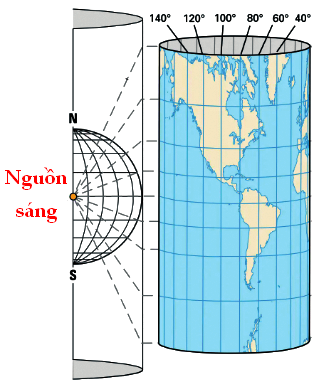
\includegraphics[scale=0.45]{hinhve/CTST/CTST-1_4_1}
}
	\loigiai{
		\immini{Vì điểm nằm cách xích đạo không quá $20$ (cm) trên bản đồ nên ta có $-20 \leq y \leq 20$.\\
			Khi đó $-20 \leq 20 \tan \left(\dfrac{\pi}{180} \varphi\right) \leq 20$ hay $-1 \leq \tan \left(\dfrac{\pi}{180} \varphi\right) \leq 1$.\\
			Ta có $-90<\varphi<90$ khi và chi khi $-\dfrac{\pi}{2}<\dfrac{\pi}{180} \varphi<\dfrac{\pi}{2}$.\\
			Xét đồ thị hàm số $y=\tan x$ trên khoảng $\left(-\dfrac{\pi}{2} ; \dfrac{\pi}{2}\right)$ (Hình vẽ bên).\\
			Ta thấy $-1 \leq \tan \left(\dfrac{\pi}{180} \varphi\right) \leq 1$ khi và chi khi $-\dfrac{\pi}{4} \leq \dfrac{\pi}{180} \varphi \leq \dfrac{\pi}{4}$ hay $-45 \leq \varphi \leq 45$.\\
			Vậy trên bản đồ, các điểm cách xích đạo không quá $20$ (cm)
			nằm ở vĩ độ từ $-45^{\circ}$ đến $45^{\circ}$.}
		{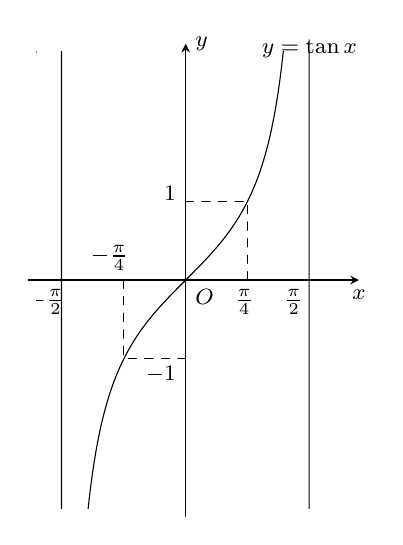
\begin{tikzpicture}[scale=1,>=stealth, font=\footnotesize, line join=round, line cap=round]
				\def\xmin{-2} \def\xmax{2.2} \def\ymin{-3} \def\ymax{3}
				\draw[->] (\xmin,0)--(\xmax,0) node [below]{$x$};
				\draw[->] (0,\ymin)--(0,\ymax) node [right]{$y$};
				\node at (0,0) [below right]{$O$};
				\node at (0.3*pi-0.1,2.7) [above right]{$y=\tan x$};
				\clip (\xmin+0.1,\ymin+0.1) rectangle (\xmax-0.5,\ymax-0.1);
				\draw[smooth,samples=400,domain=\xmin:\xmax] plot(\x,{tan(\x r)});
				\node at (0,1.1) [left]{$1$};
				\node at (0,-1.2) [left]{$-1$};
				\node at (-0.18*pi-0.4,0) [above]{$-\frac{\pi}{4}$};
				\node at (0.3*pi-0.2,0) [below]{$\frac{\pi}{4}$};
				\node at (-2*pi-0.2,0) [above]{$-2\pi$};
				\node at (-1.5*pi-0.4,0) [below]{$-\frac{3\pi}{2}$};
				\node at (-pi-0.2,0) [above]{$-\pi$};
				\node at (-0.5*pi-0.2,0) [below]{$-\frac{\pi}{2}$};
				\node at (0.5*pi-0.2,0) [below]{$\frac{\pi}{2}$};
				\node at (1.5*pi-0.3,0) [below]{$\frac{3\pi}{2}$};
				\node at (2*pi+0.2,0) [below]{$2\pi$};
				\draw[dashed] (0.25*pi,0)--(0.25*pi,1)--(0,1);
				\draw[dashed] (-0.25*pi,0)--(-0.25*pi,-1)--(0,-1);
		\end{tikzpicture}}
	}
\end{bt}

\begin{bt}%[1D1V4-7]%[BG K11, Nhật Thiện]	[Mức độ 3]
	\immini{
		Khoảng cách từ tâm một guồng nước đến mặt nước và bán kính của guồng đều bằng $3$ m. Xét gàu $G$ của guồng. Ban đầu gàu $G$ nằm ở vị trí $A$ (Hình vẽ bên).
		\begin{enumerate}
			\item Viết hàm số $h$ biểu diễn chiều cao (tính bằng mét) của gàu $G$ so với mặt nước theo góc $\alpha = \left(OA,OG\right)$.
			\item Guồng nước quay hết mỗi vòng trong $30$ giây. Dựa vào đồ thị của hàm số sin, hãy cho biết ở các thời điểm $t$ nào trong $1$ phút đầu, khoảng cách của gàu đến mặt nước bằng $1{,}5$ mét?
		\end{enumerate}
	}{
		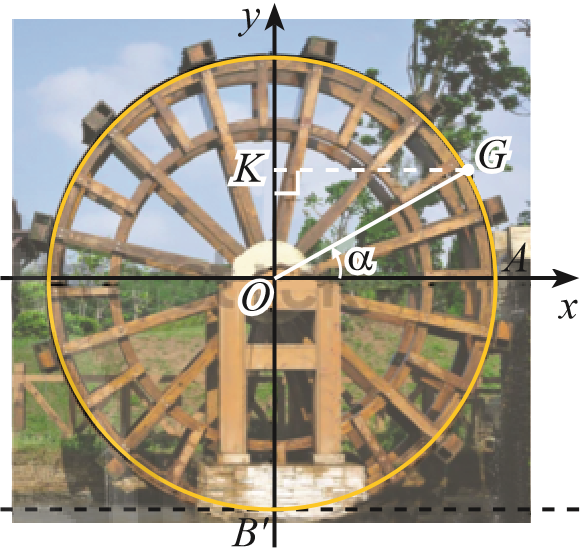
\includegraphics[scale=.6]{hinhve/CTST/CTST-1_4_3}
	}
	\loigiai{
		\begin{enumerate}
			\item Ta có chiều cao $h$ của gàu $G$ so với mặt nước là
			\[h = 3 + 3\sin\alpha\,(\text{m}).\]
			\item Vì guồng nước quay hết mỗi vòng trong 30 giây nên trong $60$ giây đầu, guồng $G$ đi được đúng $2$ vòng.\\
			Ta có đồ thị của hàm số $h$ trong $2$ chu kì đầu tiên như sau:
			\begin{center}
				\begin{tikzpicture}[>=stealth,yscale=.4]
					\draw[->](-1,0) -- (14.5,0) node[below]{\footnotesize $\alpha$};
					\draw[->](0,-1.5) -- (0,7) node[right]{\footnotesize $h_\alpha\;\left(\text{m}\right)$};
					\draw[fill = black] (0,0) node [below left]{$O$} circle (1pt);
					\draw[fill = black] (pi,0) node [below,red]{\footnotesize $\pi$ (15s)} circle (1pt) (2*pi,0) node [below,red]{\footnotesize $2\pi$ (30s)} circle (1pt) (3*pi,0) node [below,red]{\footnotesize $3\pi$ (45s)} circle (1pt) (4*pi,0) node [below,red]{\footnotesize $4\pi$ (60s)} circle (1pt);
					\draw[fill = black] (pi/2,0) node [below]{\footnotesize $\tfrac{\pi}{2}$} circle (1pt) (3*pi/2,0) node [below]{\footnotesize $\tfrac{3\pi}{2}$} circle (1pt) (5*pi/2,0) node [below]{\footnotesize $\tfrac{5\pi}{2}$} circle (1pt) (7*pi/2,0) node [below]{\footnotesize $\tfrac{7\pi}{2}$} circle (1pt);
					\draw[smooth, samples=100, domain=0:4*pi]plot(\x,{3+3*sin((\x)*180/pi)});
					\draw[dashed] (pi/2,0)--(pi/2,6) (5*pi/2,0)--(5*pi/2,6)--(0,6) node[left]{$6$} (pi,0)--(pi,3) (2*pi,0)--(2*pi,3) (3*pi,0)--(3*pi,3) (4*pi,0)--(4*pi,3)--(0,3) node[left]{$3$};
					\draw[blue,thick] (0,1.5)--(4*pi+1,1.5) node[above]{\footnotesize $h=1{,}5$};
				\end{tikzpicture}
			\end{center}
			Dựa vào đồ thị hàm số sin, ta thấy trong 2 chu kì đầu tiên thì có 4 thời điểm mà gàu $G$ cách mặt nước $1{,}5$ mét, ứng với các thời điểm $t=17{,}5$ s; $t=27{,}5$ s; $t=47{,}5$ s và $t=57{,}5$s.
		\end{enumerate}	
	}
\end{bt}

\begin{bt}%[1D1V4-7]%[BG K11, Nhật Thiện]	[Mức độ 3]
	Trong hình vẽ bên dưới, một chiếc máy bay $A$ bay ở độ cao $500$ m theo một đường thẳng đi ngang qua phía trên trạm quan sát $T$ ở mặt đất. Hình chiếu vuông góc của $A$ lên mặt đất là $H$, $\alpha$ là góc lượng giác $\left(Tx,TA\right)$ $\left(0<\alpha<\pi\right)$.
	\begin{center}
		\begin{tikzpicture}[>=stealth,x=1.0cm,y=1.0cm, scale=1]
			\draw[->](0,0) -- (14,0) node[below]{\footnotesize $x$ (m)};
			\draw[dashed,red](0,3) -- (14,3);
			\path
			(5,0) coordinate (T)
			(10,0) coordinate (H)
			(10,3) coordinate (A)
			;
			\draw[fill = black] (T) node [below]{\footnotesize$T$ (trạm quan sát)} circle (1pt) -- (H) node [below] {\footnotesize$H$} circle (1pt) -- (A) node [above]{\footnotesize$A$ (máy bay)} circle (1pt) -- (T);
			\draw (10,1.5) node [right]{\footnotesize $500$m};
			\draw pic[->,draw, angle radius=5mm]{angle=H--T--A} (T) node[shift={(10:.8)}]{$\alpha$};
			\path pic[draw,angle radius=6]{right angle=A--H--T};
		\end{tikzpicture}
	\end{center}
	\begin{enumerate}
		\item Biểu diễn tọa độ $x_H$ của điểm $H$ trên trục $Tx$ theo $\alpha$.
		\item Dựa vào đồ thị hàm số cotan, hãy cho biết với $\dfrac{\pi}{6} < \alpha < \dfrac{2\pi}{3}$ thì $x_H$ nằm trong khoảng nào? Làm tròn kết quả đến hàng phần mười.
	\end{enumerate}
	\loigiai{
		\begin{enumerate}
			\item Coi trạm quan sát $T$ là gốc tọa độ thì ta có
			\[x_H = \overline{TH} = AH\cdot\cot\alpha = 500\cot\alpha\;\left(\text{m}\right).\]
			\item \immini{
				Dựa vào đồ thị hàm số $\cot x$, ta thấy với $\dfrac{\pi}{6} < \alpha < \dfrac{2\pi}{3}$ thì $-\dfrac{\sqrt{3}}{3} < \cot \alpha < \sqrt{3}$.\\
				Do đó $-\dfrac{500\sqrt{3}}{3} < x_H < 500\sqrt{3}$. Làm tròn kết quả đến hàng phần mười ta được
				\[-288{,}7 < x_H< 866{,}0.\]
			}{
				\begin{tikzpicture}[font=\footnotesize,line join = round, line cap = round,>=stealth,scale=1]
					\draw[->] (-1,0) -- (4,0.)node[below]{\footnotesize $x$};
					\draw[->] (0,-3.1) -- (0,4.25)node[left]{\footnotesize $y$};
					\draw (0,0) node[above left] {\footnotesize $O$};
					\draw[dashed,smooth,samples=100,domain=0.25:2.8] plot(\x,{cot(((\x))*180/pi)});
					\draw[line width=1pt,smooth,red,samples=100,domain=pi/6:2*pi/3] plot(\x,{cot(((\x))*180/pi)});
					\draw[dashed] (pi,-3.1) -- (pi,0) node[below right]{$\pi$} -- (pi,4.2);
					\draw[dashed] (pi/6,0) node[below]{$\tfrac{\pi}{6}$} circle (1pt) --(pi/6,1.73)--(0,1.73) node[left]{$\sqrt{3}$};
					\draw[dashed] (2*pi/3,0) node[above]{$\tfrac{2\pi}{3}$} circle (1pt) --(2*pi/3,-0.577)--(0,-0.577) node[left]{$-\tfrac{\sqrt{3}}{3}$};
				\end{tikzpicture}
			}
		\end{enumerate}
	}
\end{bt}